\documentclass[tikz,border=2pt]{standalone}
\usepackage{amsmath,amssymb}
\usepackage{tikz}
\usetikzlibrary{arrows.meta}

\begin{document}
% Dynamic programming: stages (periods) and states (inventory levels); every arrow is a
% decision with its cost, f_i(state) is the best value of reaching the state, computed stage
% by stage and reused by every later arrow leaving the state.
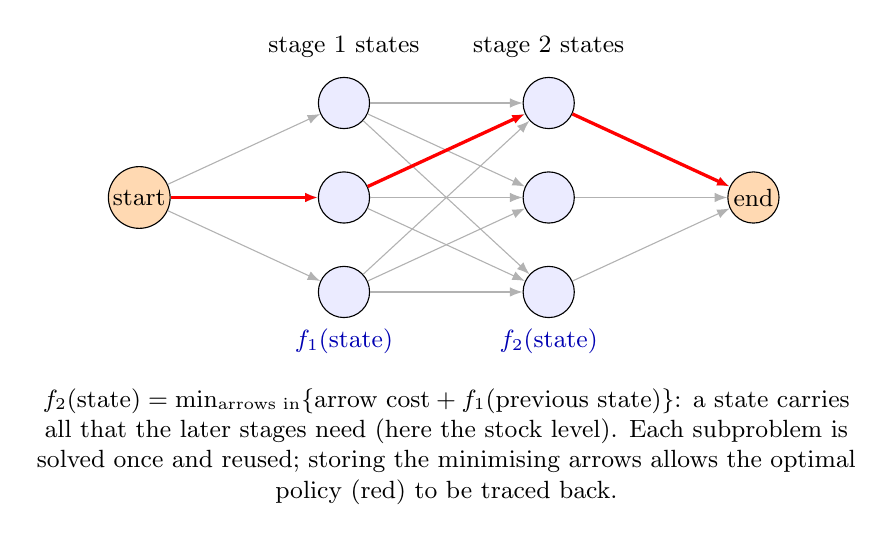
\begin{tikzpicture}[every node/.style={font=\small}, >={Latex[length=1.6mm]}, st/.style={draw, circle, minimum size=6.5mm, inner sep=1pt, fill=blue!8}]
	\node[st, fill=orange!30] (s) at (0,0) {start};
	\foreach \k in {0,1,2} {\node[st] (a\k) at (2.6,{1.2-1.2*\k}) {};}
	\foreach \k in {0,1,2} {\node[st] (b\k) at (5.2,{1.2-1.2*\k}) {};}
	\node[st, fill=orange!30] (e) at (7.8,0) {end};
	\foreach \k in {0,1,2} {\draw[->, gray!60] (s) -- (a\k);}
	\foreach \k in {0,1,2} {\foreach \l in {0,1,2} {\draw[->, gray!60] (a\k) -- (b\l);}}
	\foreach \k in {0,1,2} {\draw[->, gray!60] (b\k) -- (e);}
	\draw[->, red, very thick] (s) -- (a1); \draw[->, red, very thick] (a1) -- (b0); \draw[->, red, very thick] (b0) -- (e);
	\node[anchor=south] at (2.6,1.65) {stage 1 states};
	\node[anchor=south] at (5.2,1.65) {stage 2 states};
	\node[blue!70!black, anchor=north] at (2.6,-1.55) {$f_1(\text{state})$};
	\node[blue!70!black, anchor=north] at (5.2,-1.55) {$f_2(\text{state})$};
	\node[anchor=north, align=flush center, text width=10.4cm] at (3.9,-2.3) {$f_2(\text{state})=\min_{\text{arrows in}}\{\text{arrow cost}+f_1(\text{previous state})\}$: a state carries all that the later stages need (here the stock level). Each subproblem is solved once and reused; storing the minimising arrows allows the optimal policy (red) to be traced back.};
\end{tikzpicture}
\end{document}
